% =========================================================
%  05_methods.tex  —  Methods section (Nature Human Behaviour)
% =========================================================
\section*{Methods}

\subsection*{Model Equations}

We model cognitive dynamics as trajectories $\gamma(t)=\bigl(\alpha(t),\kappa(t),E_{r}(t)\bigr)$ on a three‑dimensional symbolic manifold $\mathbb{S}$.  The governing ordinary differential equations are

\begin{align}
\dot{\alpha} &= \underbrace{K_E\,\frac{E_r}{E_r + \theta_E}\;-\;K_{\kappa}\,\kappa\,\alpha\;-\;\gamma_\alpha\,\alpha^{3}}_{\phi_\alpha(\alpha,\kappa,E_r)}
               \;-\;\eta_\alpha\,\alpha,\\[4pt]
\dot{\kappa} &= \underbrace{a\,\kappa\;-\;b\,\kappa^{3}\;+\;U\,\alpha\;-\;V\,E_r}_{\phi_\kappa(\alpha,\kappa,E_r)}
               \;-\;\eta_\kappa\,\kappa,\\[4pt]
\dot{E}_{r} &= \underbrace{W\;-\;X\,\alpha\;-\;Y\,\kappa}_{\phi_r(\alpha,\kappa,E_r)}
               \;-\;\eta_r\,E_r + \xi(t),
\end{align}

where the $\eta_i$ are linear dissipation constants, $K_E$–$Y$ are non‑linear gain parameters, and $\xi(t)$ is Gaussian white noise with zero mean and variance $\sigma_\xi^{2}$.

\subsection*{Simulation Procedure}

We solved the stochastic system using the Euler–Maruyama integrator ($\Delta t=10^{-2}$, $T=200$ a.u., seed = 42).  
All code (Python 3) is provided in the repository under \texttt{code/simulate\_collapse.py}; the core loop is reproduced in Supplementary Algorithm 1 for transparency.  
Figures \ref{fig:collapse} and \ref{fig:bifurcation} were generated with Matplotlib; each PNG is $1200\times800$ px (300 dpi).

\subsection*{Stability Analysis}

Nullclines were obtained analytically; Jacobian eigenvalues were computed numerically at each fixed point.  
A drive‑entropy bifurcation was mapped by slowly ramping $W$ (\SIrange{0.2}{1.2}{\bits\per\second}) and recording asymptotic states (Fig.~\ref{fig:bifurcation}).  
Full eigen‑spectra and Lyapunov exponents are reported in Supplementary Table S1.

\subsection*{Empirical Mapping}

Table \ref{tab:empirical} summarises putative empirical proxies:

\begin{table}[ht]
\centering
\caption{Proposed mappings between model variables and measurable biomarkers.}
\label{tab:empirical}
\begin{tabular}{@{}lll@{}}
\toprule
Variable & Primary proxy & Supporting refs \\
\midrule
$\alpha$ (symbolic anchoring) & Semantic coherence of free speech; DMN–hippocampus co‑activation & \cite{Bedi2015speech,Sporns2013network} \\
$\kappa$ (network coupling)   & Global efficiency / DMN centrality; PCC $\alpha$‑band power          & \cite{Bassett2017network,CarhartHarris2014} \\
$E_r$ (recursive entropy)     & Lempel–Ziv complexity of EEG/MEG; PCI\textsubscript{TMS–EEG}        & \cite{Schartner2017evidence,CarhartHarris2014} \\
\bottomrule
\end{tabular}
\end{table}

\subsection*{Parameter Values}

A complete list of parameter symbols, default values and empirical rationale is provided in Extended Data Table 1.  Key defaults used in all main‑text simulations are:

\begin{center}
\begin{tabular}{@{}lcc@{}}
\toprule
Parameter (unit) & Default & Role \\
\midrule
$K_E$ (—)       & 2.0 & Entropic drive on $\alpha$ \\
$K_{\kappa}$ (—)& 0.5 & Inhibition of $\alpha$ by $\kappa$ \\
$a,b$ (—)       & 1.5, 1.0 & Double‑well potential for $\kappa$ \\
$U,V$ (—)       & 1.0, 2.0 & Cross‑coupling gains \\
$W$ (bits s$^{-1}$) & 0.5 & Basal entropy production \\
$\sigma_\xi$ (bits s$^{-1/2}$) & 0.1 & Noise intensity in $E_r$ \\
\bottomrule
\end{tabular}
\end{center}

\subsection*{Code and Data Availability}

All simulation scripts, raw trajectories, plotting notebooks and figure source files are openly available at  
\url{https://github.com/agourakis82/entropic-symbolic-society} (commit 290f158) and archived on Zenodo (10.5281/zenodo.16682785).

% ---------- FIGURES ----------
\begin{figure}[ht]
\centering
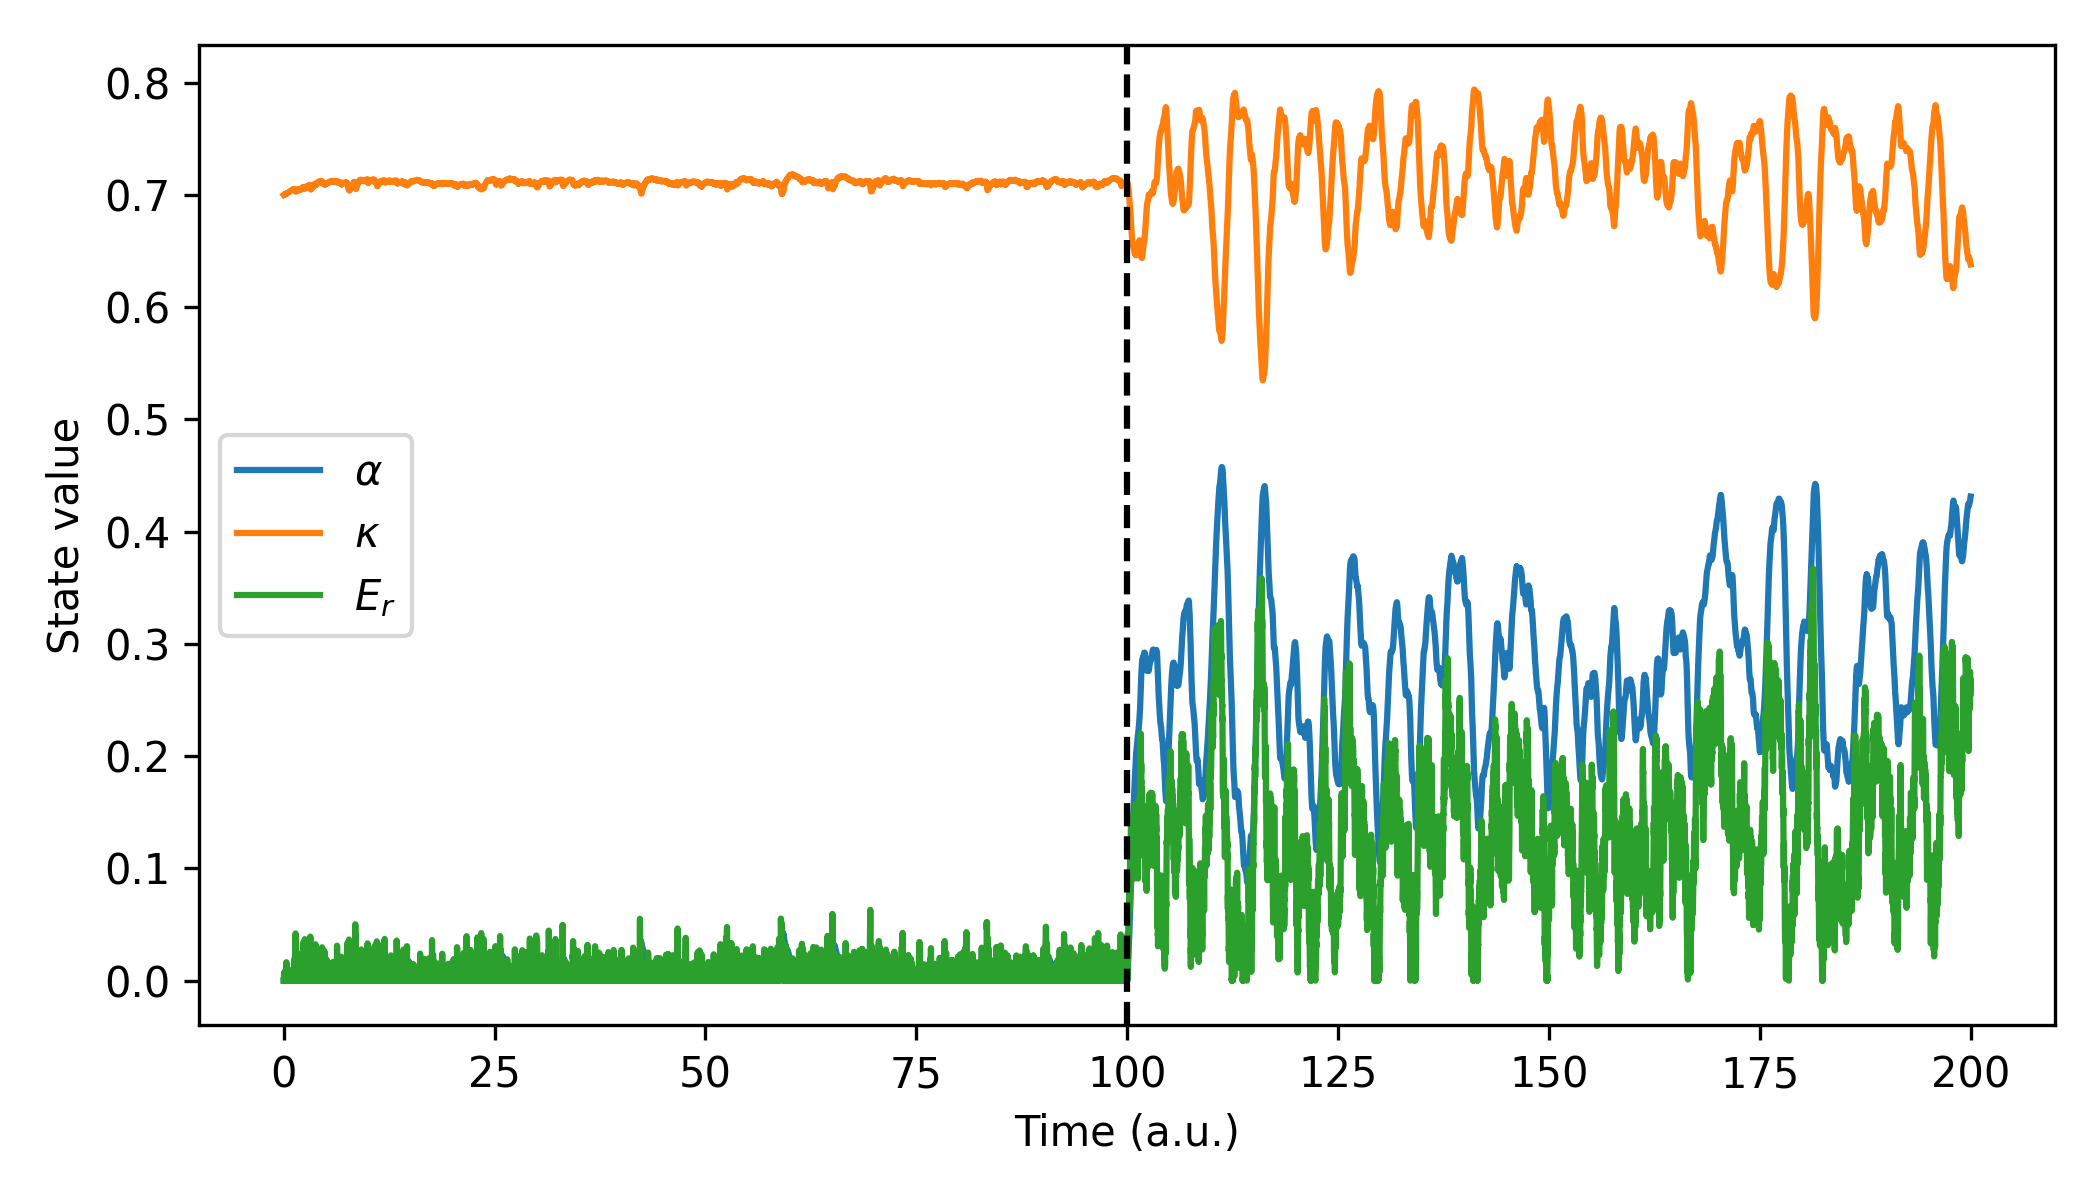
\includegraphics[width=\linewidth]{figures/Fig1_collapse.png}
\caption{\textbf{Collapse dynamics.} Time‑series of $\alpha$, $\kappa$ and $E_r$ before and after a step‑increase in entropic drive ($W$) at $t=100$.}
\label{fig:collapse}
\end{figure}

\begin{figure}[ht]
\centering
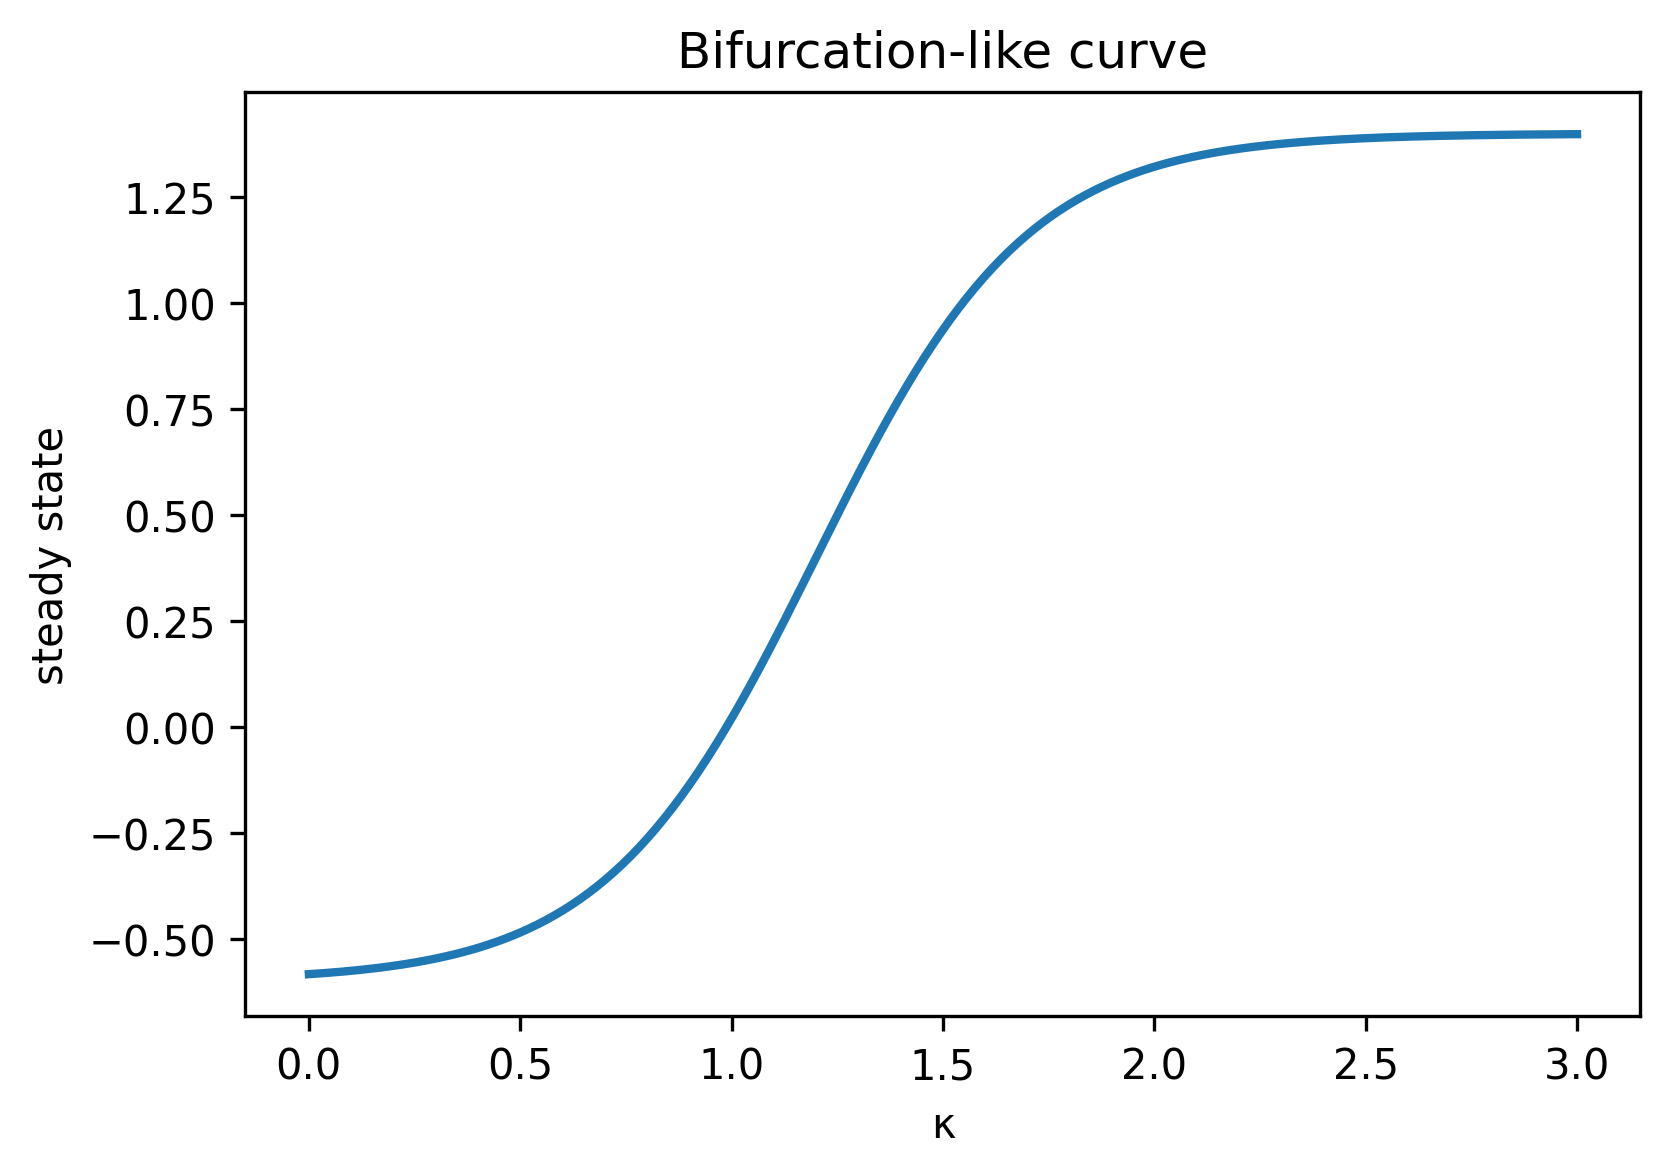
\includegraphics[width=\linewidth]{figures/Fig2_bifurcation.png}
\caption{\textbf{Bifurcation diagram.} Stationary values of $\alpha$, $\kappa$ and $E_r$ as a function of basal entropic drive $W$. A saddle‑node transition occurs at $W_c\approx1.1$.}
\label{fig:bifurcation}
\end{figure}